% R2: separability analysis (Sanika). Numbers from scripts/run_analysis.py, seed 0;
% figures and tables from scripts/make_report_figures.py.
% Needs: graphicx, booktabs, amsmath. Paths assume the main .tex file lives in report/.

\section{Separability Analysis}\label{sec:separability}

\textit{Which features separate which classes on recordings the model has not seen?}
For each of the 126 features and each of the 15 class pairs we compute the two-class
Fisher ratio on held-out recordings: the class means come from the training fold and the
within-class spread from the held-out windows around those means. We report the median
over the six grouped folds, because each fold holds out only one recording per class, and
a recording that happens to sit next to the training mean can make one fold's $J$ explode
(one fold reached 88 where the others gave 0.5--2). For whole-pair separability we project
onto the two-class LDA direction fitted on the training fold and score the held-out windows
along it. Along that direction the in-sample $J$ is 600--1600 for every pair, while the
held-out $J$ is 0.4--7.4 (Fig.~\ref{fig:pairj}): LDA mostly learns which recording a window
came from. All numbers are single-seed (seed 0).

\begin{figure}[t]
  \centering
  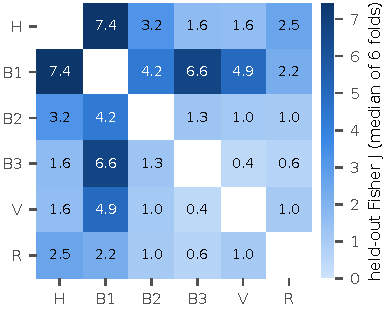
\includegraphics[width=0.8\columnwidth]{figures/fig_pair_j.pdf}
  \caption{Held-out Fisher $J$ for every class pair, along the pair's LDA direction (median
  of 6 grouped folds). B1 separates from every class; B2, B3, V and R form a confusable
  block.}
  \label{fig:pairj}
\end{figure}

\textbf{B1 separates from everything, through impulsiveness.} B1 is the only class with
held-out $J>2$ against all five others (2.2--7.4). Against H the strongest features are
kurtosis ($J=7.5$, worst fold 1.3), peak-to-peak (4.7) and impulse factor (4.1):
insufficient lubrication makes the vibration impulsive, and time-domain statistics capture
that without any defect frequency, as hypothesised. No single feature separates any class
from all five others (the best weakest-pair $J$ is 0.76, for V), so separation always needs
combinations of features.

\textbf{R is not separated by its rotor-bar sidebands.} We expected R to be easy, since the
pole-pass sidebands at $f_1 \pm f_p$, $f_p = 2 s f_\text{supply}$, lie well below Nyquist.
Three checks say otherwise (Fig.~\ref{fig:sidebands}).
(i)~The hand-written sideband feature integrates 0.5--3\,Hz either side of $f_1$, but the
measured $f_p$ is 3.5--10.1\,Hz under load (slip 4--10\% at reduced supply frequency) and
below 0.5\,Hz unloaded, so the real sidebands fall inside the band in 0 of 36 recordings.
(ii)~Measured directly at $f_1 \pm f_p$ on a 0.012\,Hz spectrum, R's sidebands are never the
strongest at their condition (rank 3, 6 and 4 of 6 under load at 30, 40, 50\,Hz).
(iii)~At 50\,Hz supply the sideband positions coincide with aliased shaft harmonics for
\emph{any} slip: for a 4-pole motor $f_1 + f_p = 2f_\text{supply} - 3f_1 = 100 - 3f_1$,
the alias of $3f_1$, and $f_1 - f_p$ is the alias of $5f_1$. A 100\,Hz sensor cannot tell
rotor-bar sidebands from running-speed harmonics there.
R's one consistent signature is slip: under load it has the second-highest slip at every
speed (median 0.056 against 0.043--0.047 for H and the bearing classes), consistent with the
torque lost to broken bars. Unloaded, however, every class slips about 0.2\%, so pooled
over conditions slip barely separates R, and the best single R--B2 feature reaches a median
$J$ of only 0.75 (worst fold 0.01). This is the R$\leftrightarrow$B2 confusion in the
baseline.

\begin{figure*}[t]
  \centering
  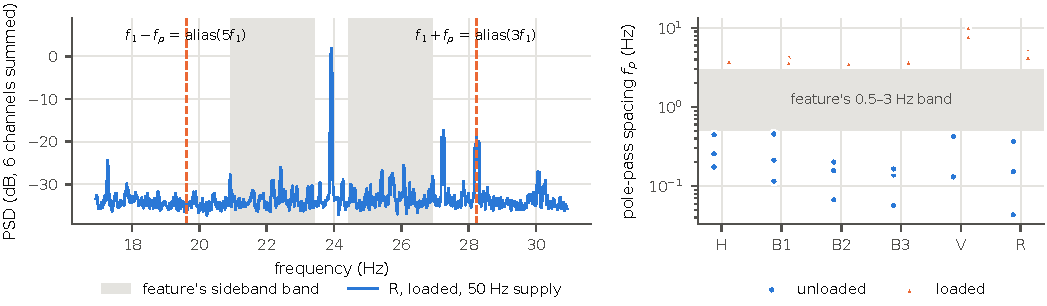
\includegraphics[width=\textwidth]{figures/fig_sidebands.pdf}
  \caption{Left: spectrum of the loaded R recording at 50\,Hz supply. The predicted
  rotor-bar sidebands (dashed) fall outside the band the sideband feature integrates
  (grey) and coincide with the aliases of $5f_1$ and $3f_1$. Right: pole-pass spacing
  $f_p$ of all 36 recordings; none falls in the feature's 0.5--3\,Hz band.}
  \label{fig:sidebands}
\end{figure*}

\textbf{B3 and V: secondary effects, plus some aliased energy.} The defining frequencies of
B3 (outer-race defect) and V (twice line frequency) lie above 50\,Hz. To see where any
separability comes from, we split each window's spectrum, relative to its own running
speed $f_1$, into sub-synchronous energy, in-band shaft harmonics, aliases of shaft
harmonics above 50\,Hz, aliases of line harmonics, and the remainder, and score each
region's energy share like a feature (Fig.~\ref{fig:regions}).
The strong 28 and 42\,Hz peaks of the loaded 30\,Hz recordings are not aliasing: in every
class they sit at exactly $2f_1$ and $3f_1$ ($f_1\approx14$\,Hz), in band and present in
H as well, so they are not specific to any class.
V's own signature is nearly invisible. Twice line frequency folds to DC at 50\,Hz supply,
where it is removed with the mean; at 40\,Hz it lands on the running speed; only at 30\,Hz
does it appear on a separate bin (40\,Hz), and even there it gives $J=1.27$ against H
(two usable folds).
The best single measure for H versus V is instead the energy at aliased
\emph{shaft}-harmonic positions ($J=2.75$): H keeps about 8\% of its energy there and V
about 1\%. Part of V's separability therefore does rest on aliased energy, but on
mechanical harmonics folded down from above Nyquist rather than on V's own signature.
Under load V also slips far more than any other class (median 0.101), a low-frequency
effect of the reduced torque that shifts its whole harmonic comb, while its total level
differs from H by at most about 2\,dB.
B3 has no spectral region that separates it from H (every region $J \le 0.21$); its best
single feature is time-domain skewness ($J=1.11$), i.e.\ waveform asymmetry rather than a
spectral line. Of the B3 peaks standing at least 10\,dB above H at the same condition,
9 of 15 match no shaft, line or bearing frequency, either directly or as an alias, and
only 3 are aliases (Table~\ref{tab:peaks}). We assumed 6204-type bearing factors because
the dataset does not name the bearing, so unexplained peaks may still be defect lines.

\begin{figure}[t]
  \centering
  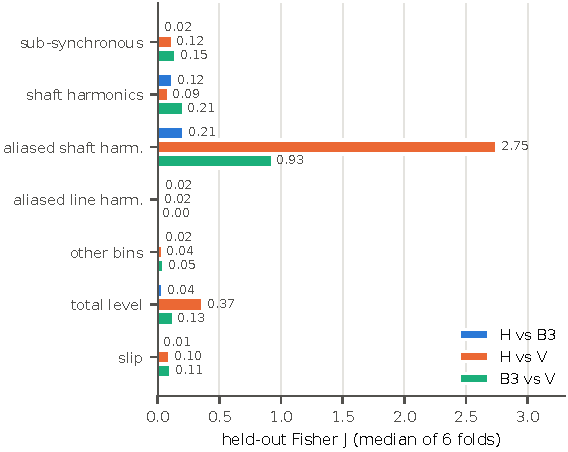
\includegraphics[width=\columnwidth]{figures/fig_regions.pdf}
  \caption{Held-out Fisher $J$ of the energy share in each spectral region, plus total
  level and slip, for the pairs involving B3 and V.}
  \label{fig:regions}
\end{figure}

\begin{table}[t]
  \centering
  \caption{Peaks of B3 and V at least 10\,dB above H at the same condition, by the source
  they match.}
  \label{tab:peaks}
  \begin{tabular}{lrrrr}
\toprule
Class & in-band shaft & aliased & unexplained & total \\
\midrule
B3 & 3 & 3 & 9 & 15 \\
V & 7 & 4 & 26 & 37 \\
\bottomrule
\end{tabular}

\end{table}

\textbf{Summary.} The separability that survives the 100\,Hz sensor is mostly not the
textbook signatures. Lubrication loss survives through impulsiveness. The rotor-bar
signature is missed by the feature at every speed and, at 50\,Hz supply, cannot be
separated from aliased harmonics at all. V and B3 are told apart, weakly, by slip, waveform
shape and aliased mechanical harmonics, not by their defining frequencies.
